\section{The braiding in the Hall algebra}
\label{BraidingHallAlgebra}
Here we explain how the extended Waldhausen construction produces a braiding.

Given a category $\CCC$ \adam{satisfying...} we construct the geometric Hall algebra $H_{geom}$ of $\CCC$ as in \autoref{GeneralHall} and compose it with $T^C$ from \autoref{CatTransfer} to get a functor $H_{\CCC}:\AugOrdSet\otimes\AugOrdSet\to\LinCat$. Denote $\HH:=H_\CCC(\ord{1})$.

The restriction of $H_{\CCC}$ to $\{1\}\otimes\AugOrdSet$ gives us a monoidal structure on $\HH$.

\begin{Theorem}
$H_\CCC$ induces a braiding on $\HH$.
\end{Theorem}

\begin{Example}
\label{VectHallExample}
For $\CCC=\Vect_\field$, $H_{\CCC}(\ord{1})\cong\bigoplus \Rep(\GL(n,\field))$
\end{Example}

Consider the image under $H_{geom}$ of the square in $\AugOrdSet\otimes\AugOrdSet$
\begin{equation}
\label{HopfSquare}
\stik{1}{
(\ord{2},\ord{2}) \ar{d}{} \ar{r}{} \& (\ord{2},\ord{1}) \ar{d}{} \\
(\ord{1},\ord{2}) \ar{r}{} \& (\ord{1},\ord{1})
}
\end{equation}

The image of this square under $H_{geom}$ is a square with a 2-morphism. It can be described pictorially as follows:

If we present the correspondence 
\[
\stik{1}{
{} \& S_2 \ar{dl}[above]{end} \ar{dr}{mid} \& {} \\
S_1\times S_1 \& {} \& S_1
}
\]
from \autoref{HallAlgebra} which gives the multiplication in the Hall algebra as the picture
\[

\includegraphics{Figures/HallMultPictorial.pdf}
\]

Then the image of the square is
\[
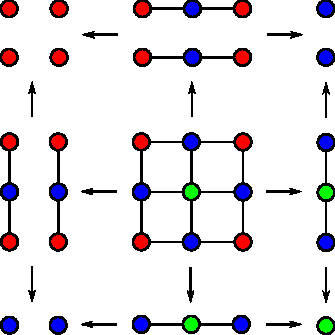
\includegraphics{Figures/HallHopfPictorial.pdf}
\]
The stack in the center of this square giving the 2-morphism is a grid of exact sequences with the obvious projections. We show how to get this square below in \autoref{Extension}.

Applying $T^C$, this gives a 2-morphism
\[
\stik{1}{
    \HH^{\otimes 4} \ar{r}{} \ar{d}{} \& \HH^{\otimes 2} \ar{d}{} \ar[Rightarrow, shorten <=1em,shorten >=1em]{dl}{}\\
    \HH^{\otimes 2} \ar{r}{} \& \HH
}
\]

If we restrict to objects of the form $1\otimes A\otimes B \otimes 1$ this gives a morphism $c_{A,B}:m(A,B)\to m(B,A)$ which is a candidate for a braiding.

\begin{Proposition}
\label{Thm:braiding}
$c_{A,B}$ defines a braiding on $\HH$
\end{Proposition}

The rest of this section is a sketch for a proof of \autoref{Thm:braiding}.
A rigorous treatment will be given in \cite{GeometricHallAlgebra2} where this result will follow from a more general result about the extended combinatorial Hall algebra construction.

As discussed in \autoref{BraidingGeneral}, we need to show that the cube \autoref{HexagonCube} constructed from the braiding and the associator, is commutative.

This cube is the image of the cube in $\AugOrdSet\otimes\AugOrdSet$:
\begin{equation}
\label{braidingcubeInDelta}
\stik{1}{
 \& (\ord{2},\ord{2}) \ar{rr} \ar{dd} \& {} \& (\ord{2},\ord{1}) \ar{dd}\\
(\ord{3},\ord{2}) \ar[crossing over]{rr} \ar{dd} \ar{ur} \& {} \& (\ord{3},\ord{1}) \ar{dd} \ar{ur} \& {}\\
{} \& (\ord{1},\ord{2}) \ar{rr} \& {} \& (\ord{1},\ord{1})\\
(\ord{2},\ord{2}) \ar{rr} \ar{ur} \& {} \& (\ord{2},\ord{1}) \ar{ur}
\latearrow{commutative diagrams/crossing over}{2-3}{4-3}{}
}
\end{equation}

We shall show that its image commutes already on the level of $H_{geo}$. That is, $H_{geo}$ produces for us a cube of correspondences, and in order for its image under $T^C$ to commute it is sufficient to show that the cubes in its upper-right-back and lower-left-front corners are pullback cubes (see \autoref{CorrCubeCommute}). Our main technical tool will be \autoref{PullbackCubeLemma}.

Let's consider first the lower-left-front cube. 

\begin{Claim}
\label{Lem:LeftFace}
Its left face is a pullback square
\end{Claim}

The underlying reason for this is that the left face of the original cube \autoref{braidingcubeInDelta} is the tensor of the associator square with itself.

Using this, and \autoref{PullbackCubeLemma}, we only need to prove that the right face is a pullback to get that the cube is a pullback.

A similar argument for the upper-right-back cube leads us to another inner square that we need to show is a pullback. In both cases these squares turn out to come from associator squares for the geometric Hall algebra associated to the category of short exact sequences in our original category. They are exactly the two squares that are pullbacks and correspond to the 2-Segal condition, as discussed in \cite[\S 4.5]{GeometricHallAlgebra1}.

\subsection{Recovering the braiding of Joyal and Street}

Here we consider the case $\CCC=\Vect_\field$. As noted in \autoref{VectHallExample}, in this case $\HH\cong\bigoplus \Rep(\GL(n,\field))$. More precisely, $H_{geom}(\ord{1})$ is the stack of vector spaces, so $\HH$ is really naturally the category of representations of the $\field$ points of this groupoid, which is what is called the category of linear species in \cite{Joyal-StreetGLn}.

\subsubsection{The monoidal structure}

The monoidal structure is given by $H_\CCC(\ord{2}\to\ord{1})$. Since $H_{geom}(\ord{2})$ is the stack of pairs of vector spaces, we have a canonical identification $H_\CCC(2)\cong\HH\otimes\HH$. Then, considering the diagram \autoref{HallMultCorrespondence} and using \autoref{GroupoidRep}, the monoidal structure $m$ is then given by the formula (for $\Phi,\Psi\in\HH$)
\[
m(\Phi,\Psi)(V)=\bigoplus_{[U\to V\to W]}\Phi(U)\otimes\Psi(W)
\]

where the sum goes over the isomorphism classes of the 2-fiber of the groupoid of short exact sequences in $\Vect_\field$ over the underlying groupoid of $\Vect_\field$ with respect to the map $mid$. A simple computation shows that this is in bijection with the set of subspaces $U\subseteq V$ so this is the same monoidal structure considered in \cite{Joyal-StreetGLn}.

\subsubsection{The braiding}

First consider the map of stacks $i:H_{geom}(\ord{2})\to H_{geom}(\ord{4})$ which sends a pair of vector spaces $(U,V)$ to the quadruple of vector spaces $(0,U,V,0)$.

We note that $T^C(i)$ implements the imbedding $\HH\otimes\HH\to\HH^{\otimes 4}, A\otimes B\mapsto \monunit\otimes A\otimes B \otimes \monunit$.

So in order to compute the braiding we need to apply $T^C$ to the diagram 
\[
%% Creator: Inkscape inkscape 0.91, www.inkscape.org
%% PDF/EPS/PS + LaTeX output extension by Johan Engelen, 2010
%% Accompanies image file 'HallBraidPictorial.pdf' (pdf, eps, ps)
%%
%% To include the image in your LaTeX document, write
%%   \input{<filename>.pdf_tex}
%%  instead of
%%   \includegraphics{<filename>.pdf}
%% To scale the image, write
%%   \def\svgwidth{<desired width>}
%%   \input{<filename>.pdf_tex}
%%  instead of
%%   \includegraphics[width=<desired width>]{<filename>.pdf}
%%
%% Images with a different path to the parent latex file can
%% be accessed with the `import' package (which may need to be
%% installed) using
%%   \usepackage{import}
%% in the preamble, and then including the image with
%%   \import{<path to file>}{<filename>.pdf_tex}
%% Alternatively, one can specify
%%   \graphicspath{{<path to file>/}}
%% 
%% For more information, please see info/svg-inkscape on CTAN:
%%   http://tug.ctan.org/tex-archive/info/svg-inkscape
%%
\begingroup%
  \makeatletter%
  \providecommand\color[2][]{%
    \errmessage{(Inkscape) Color is used for the text in Inkscape, but the package 'color.sty' is not loaded}%
    \renewcommand\color[2][]{}%
  }%
  \providecommand\transparent[1]{%
    \errmessage{(Inkscape) Transparency is used (non-zero) for the text in Inkscape, but the package 'transparent.sty' is not loaded}%
    \renewcommand\transparent[1]{}%
  }%
  \providecommand\rotatebox[2]{#2}%
  \ifx\svgwidth\undefined%
    \setlength{\unitlength}{204.73104642bp}%
    \ifx\svgscale\undefined%
      \relax%
    \else%
      \setlength{\unitlength}{\unitlength * \real{\svgscale}}%
    \fi%
  \else%
    \setlength{\unitlength}{\svgwidth}%
  \fi%
  \global\let\svgwidth\undefined%
  \global\let\svgscale\undefined%
  \makeatother%
  \begin{picture}(1,0.97111946)%
    \put(0,0){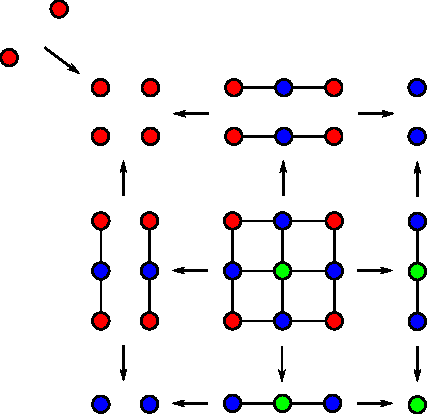
\includegraphics[width=\unitlength,page=1]{Figures/HallBraidPictorial.pdf}}%
    \put(0.13004064,0.83910531){\color[rgb]{0,0,0}\makebox(0,0)[lb]{\smash{$i$}}}%
  \end{picture}%
\endgroup%

\]

This is the same as computing the 2-morphism in the square, but replacing all stacks with the ones where the upper-left and lower-right red dots correspond to the 0 object. This gives rise to the diagram

\[
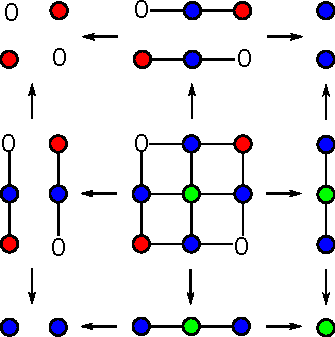
\includegraphics{Figures/HallBraidPictorialReduced.pdf}
\]

Noting that a short exact sequence starting or ending with 0 is just an isomorphism, this reduces to the following correspondence of correspondences:
\[
\stik{1}{
{} \& S_2 \ar{dl}[above]{end} \ar{dr}{mid} \& {} \\
S_1\times S_1 \& E \ar{u}{vert} \ar{d}{hor} \& S_1\\
{} \& S_2 \ar{ul}[below]{end^{op}} \ar{ur}[below]{mid} \& {}
}
\]

where $E$ is the groupoid of diagrams of the form
\[
\stik{1}{
    {} \& U \ar{d} \ar{r}{\sim} \& U' \ar{d}[above,sloped]{\sim} \\
    W \ar{r}{} \ar{d}[above,sloped]{\sim} \& V \ar{r}{} \ar{d}{} \& U'' \\
    W' \ar{r}{\sim} \& W''
}
\]

with the horizontal and vertical mid lines being short exact sequences.

The isomorphism classes of the fiber of $E$ over $(U\to V\to W)\in S_2$ are in bijection with the set of subspaces in $V$ complementary to $U$. Using this, and \autoref{GroupoidRep}, we can compute that the 2-morphism is
\begin{align*}
    m(\Phi,\Psi)(V)&=\bigoplus_{U\subseteq V}\Phi(U)\otimes\Psi(V/U) \\
    &\xrightarrow{\epsilon} \bigoplus_{U\subseteq V}\bigoplus_{W\subseteq V,U\oplus W=V} \Phi(U)\otimes\Psi(V/U) \\
    &\xrightarrow{\alpha} \bigoplus_{U\subseteq V}\bigoplus_{W\subseteq V,U\oplus W=V} \Phi(V/W)\otimes\Psi(W) \\
    &\xrightarrow{\eta} \bigoplus_{W\subseteq V} \Phi(V/W)\otimes\Psi(W) \\
    &\cong m(\Psi,\Phi)(V)
\end{align*}

with $\epsilon,\eta$ being the obvious diagonal and codiagonal maps, and $\alpha$ induced by the canonical isomorphisms $U\cong V/W,V/U\cong W$.

Up to reordering the terms in the tensor product, this is exactly the braiding of \cite{Joyal-StreetGLn}.